\section{Putnam 2005}
\textbf{Solução 1(by Sofia):}
\newline
Note que
$$\int_0^1\frac{\ln(x+1)}{x^2+1}dx=\int_0^1\sum_{n=1}^\infty \frac{(-1)^{n+1}}{n}\frac{x^n}{x^2+1}dx$$

$$=\sum_{n=1}^\infty\frac{(-1)^{n+1}}{n}\int_0^1 \frac{x^n}{x^2+1}dx$$

Defina

$$J_n=\int_0^1 \frac{x^n}{x^2+1}dx$$

$$\int_0^1\frac{\ln(x+1)}{x^2+1}dx=\sum_{n=1}^\infty\frac{(-1)^{n+1}}{n}J_n$$

então

$$J_n+J_{n+2}=\int_0^1 x^n dx=\frac{1}{n+1}.$$

$$J_0=\frac\pi 4$$

$$J_1=\frac{\log(2)}{2}$$

$$J_{2n}=(-1)^n\left(\frac\pi 4-\sum_{h=1}^n\frac{(-1)^{h+1}}{2h-1}\right)$$

$$J_{2n+1}=(-1)^n\left(\frac{\log(2)}{2}-\sum_{h=1}^n\frac{(-1)^{h+1}}{2h}\right)$$

\newline
\textbf{Solução 2 (by Libardi):}
\newline
Defina a função $I:\mathbb{R}\rightarrow\mathbb{R}$ de tal forma que:

$$I(t) = \int_0^t\frac{\ln(tx+1)}{x^2+1}dx$$

Trivialmente, temos $I(0) = 0$ e:

$$\Rightarrow \; \frac{dI}{dt} = \int_0^t\frac{x}{(tx+1)(x^2+1)}dx+\frac{\ln(t^2+1)}{t^2+1}$$

Fazendo frações parciais, determina-se $\frac{dI}{dt}$:

$$\frac{dI}{dt} = \frac{1}{t^2+1}\int_0^t\left(\frac{x+t}{x^2+1}-\frac{t}{tx+1}\right)dx+\frac{\ln(t^2+1)}{t^2+1}$$

$$\Leftrightarrow \frac{dI}{dt} = \frac{\ln(x^2+1)+2t\arctan(x)-2\ln(tx+1)}{2(t^2+1)}\Big|_{x=0}^{x=t} + \frac{\ln(t^2+1)}{t^2+1}$$

$$\Leftrightarrow \frac{dI}{dt} = \frac{t\arctan(x)}{t^2+1} + \frac{\ln(t^2+1)}{2(t^2+1)}$$

Para obter a integral desejada, integra-se $I'(t)$:

$$\int \frac{dI}{dt}dt = \int\left(\frac{t\arctan(x)}{t^2+1} + \frac{\ln(t^2+1)}{2(t^2+1)}\right)dt = \frac{1}{2}\arctan(t)\ln(1+t^2) + C$$

Portanto, como temos a condição de contorno $I(0) = 0$, conclui-se que:

$$I(t) = \frac{1}{2}\arctan(t)\ln(1+t^2)$$

Queremos saber o valor de $I(1)$:

$$I(1) = \int_0^1\frac{\ln(x+1)}{x^2+1}dx = \frac{\pi}{8}\ln(2)$$

Como queríamos demonstrar.
\newline \newline
\textbf{Solução meme (by Libardi):}
\newline
Defina a função $I:\mathbb{R}^2\rightarrow\mathbb{R}^2$ de forma que:
$$I(u,v) = \int_0^u\frac{\ln(vx+1)}{x^2+1}dx$$
Trivialmente, temos as condições de contorno $I(0,v) = 0, \forall v\in\mathbb{R}$ e $I(u,0) = 0, \forall u\in\mathbb{R}$. Ademais, temos que as derivadas parciais de primeira ordem de $I$ são:

$$\frac{\partial I}{\partial u} = \frac{\ln(uv+1)}{u^2+1}$$

$$\frac{\partial I}{\partial v} = \frac{\ln(u^2+1)+2v\arctan(u)-2\ln(uv+1)}{2(1+v^2)}$$

Com isso, montamos a equação diferencial parcial:

$$(1+u^2)\frac{\partial I}{\partial u}+(1+v^2)\frac{\partial I}{\partial v} = \frac{1}{2}\ln(u^2+1)+v\arctan(v)$$

Para resolvê-la, performa-se a transformada $(u,v)\rightarrow(\xi,\omega)$ tal que $\xi = u$ e $\omega = \arctan(v)-\arctan(u)$, com a qual se obtém:

$$(1+\xi^2)\frac{\partial I}{\partial \xi} = \frac{1}{2}\ln(\xi^2+1)+\tan(\omega+\arctan(\xi))\arctan(\xi)$$

$$\Rightarrow I = \int_0^u\left(\frac{\ln(\xi^2+1)+2\tan(\omega+\arctan(\xi))\arctan(\xi)}{2(\xi^2+1)}\right) d\xi$$

Haja vista que $\int\frac{\ln(\xi^2+1)}{\xi^2+1}d\xi = \arctan(\xi)\ln(\xi^2+1)-2\int\frac{\xi\arctan(\xi)}{\xi^2+1}d\xi$, temos:

$$I = \frac{1}{2}\arctan(u)\ln(u^2+1)+\int_0^u\frac{\arctan(\xi)}{\xi^2+1}\left(\frac{\tan(\omega)+\xi}{1-\tan(\omega)\xi} - \xi\right)d\xi$$

$$\Leftrightarrow\hspace{0.5cm} I=\frac{1}{2}\arctan(u)\ln(u^2+1)+\tan(\omega)\int_0^u\frac{\arctan(\xi)}{1-\tan(\omega)\xi}d\xi$$

Finalmente, sabendo que $\tan(\omega)\int\frac{\arctan(\xi)}{1-\tan(\omega)\xi}d\xi=-\arctan(\xi)\ln(1-\tan(\omega)\xi)+\int\frac{(\ln(1-\tan(\omega)\xi)}{\xi^2+1}d\xi$, concluímos o problema:

$$\Rightarrow I=\frac{1}{2}\arctan(u)\ln(u^2+1)-\arctan(u)\ln(1-\tan(\omega)u) + \int_0^u\frac{\ln(1-\tan(\omega)\xi)}{1+\xi^2}d\xi$$

$$\Leftrightarrow\; I(u,v)=\frac{1}{2}\arctan(u)\ln(u^2+1)-\arctan(u)\ln\left(1-\frac{u-v}{1+uv}u\right) + I\left(u,\frac{u-v}{1+uv}\right)$$

pois $\tan(\omega)=\frac{v-u}{1+uv}$, e agora simplifica-se a expressão:

$$\Leftrightarrow\; I(u,v)=\arctan(u)\ln\left(\frac{1+uv}{\sqrt{1+u^2}}\right)+I\left(u,\frac{u-v}{1+uv}\right)$$

Substituindo $u=v=1$, calcula-se a integral desejada:

$$I(1,1) = \int_0^1\frac{\ln(x+1)}{x^2+1}dx = \frac{\pi}{8}\ln(2)$$

Como queríamos demonstrar.



\section{Revista do Professor de Matemática 103 problema 454}

\begin{center}
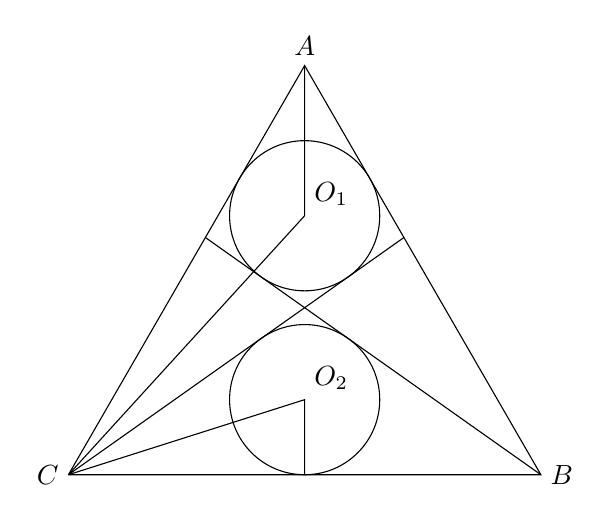
\begin{tikzpicture}[scale=3]

\draw (-1,0) node[left] {$C$}-- (1,0) node[right] {$B$} -- (0, 1.73205) node[above] {$A$}-- (-1,0);
\draw (0,1.09637) circle (0.317837);
\draw (0,0.31783) circle (0.317837);
\draw (-1,0) -- (0.42020,1.0042);
\draw (1,0) -- (-0.42020,1.0042);

\draw (-1,0) -- (0,1.09637) node[above right] {$O_1$} -- (0, 1.73205);
\draw (-1,0) -- (0,0.31783) node[above right] {$O_2$} -- (0,0);

\end{tikzpicture}
\end{center}

Dando os nomes $\alpha$ ao angulo $O_2CB$ e $\beta$ para $ACO_1$, temos que $\alpha+\beta=30^\circ$. Chame de $P_1$ e $P_2$ os pés das alturas dos triângulos $ACO_1$ e $O_2CB$ relativas aos lados $AC$ e $CB$ e $r$ o raio das esferas.

Pelo triângulo $CO_2P_2$:

$$\tan(\alpha)=r$$

e como o ângulo $AP_1O_1$ é $30^\circ$, a distância $AP_1$ é $r\sqrt{3}$, então no triangulo $CP_1O_1$

$$\tan(\beta)=\frac{r}{2-r\sqrt{3}}.$$

Agora basta resolver as equações. Temos que

$$\tan\left(\frac\pi 6-x\right)=\frac{1-\sqrt{3}\tan(x)}{\sqrt{3}+\tan(x)}$$

então

$$\frac{1-r\sqrt{3}}{\sqrt{3}+r}=\frac{r}{2-r\sqrt{3}}$$

$$r=\sqrt{3}-\sqrt{2}.$$

\section{Putnam and Beyond 1.1.3 (generalizado)}

\section{Revista do Professor de Matemática 103 problema 453/Dissertação lokona (generalizado)}

Nomeando as raízes do polinômio $x_1,x_2\dots x_{2021}$, por uma das relações de Viète temos

$$\sum_{h=1}^{2021}x_h=12126$$

$$\frac 1{2021}\sum_{h=1}^{2021}x_h=6$$

Agora trocando as variáveis for $y_i=7-x_i$. Suponha agora que o polinômio não tem raízes maiores que 7, então todos os $y_i$ são positivos.

$$\frac 1{2021}\sum_{h=1}^{2021}y_h=1$$

e

$$P(7)=\prod_{h=1}^{2021}y_h$$

$$P(7)^{1/2021}=\prod_{h=1}^{2021}y_h^{1/2021}$$

Então pela desigualdade das médias aritmética e geométrica

$$1\geq P(7)^{1/2021}$$

$$P(7)\leq 1$$

Contradizendo o enunciado. Portanto nossa suposição que todas as raízes são menores que 7 é falsa.

\section{Revista do Professor de Matemática 103 problema 452 (generalizado)}

Definindo $n+1=a^2$, $\frac n2 +1=b^2$ temos

$$a^2-2b^2=-1$$

que é uma equação de Pell negativa. Suas soluções são dadas por

$$a+b\sqrt{2}=(1+\sqrt{2})^k$$

onde $k$ é um inteiro impar. 